\section{ProductView}
\label{productview}

Im Product-View werden alle zum Kauf erhältlichen Produkte, die bei App-Start in der Liste des
\nameref{productcontroller}-Controllers gespeichert werden, in Form von individualisierten Card-Widgets angezeigt.

\subsection{Render-Widget für einzelne Produkte}

Ein Produkt wird im Product-View mittels einer Kachel dargestellt. Auf dieser befindet sich 
das Bild des Produkts, dessen Name sowie sein Preis.

Hierfür wird erneut das Card-Widget des Material-Katalogs verwendet.

Nach bereits bekanntem Prinzip muss dem Konstruktor des Custom-Widgets ein Produkt-Objekt
übergeben werden, aus welchem alle erforderlichen Daten wie

\begin{itemize}
    \item das Bild des Produkts
    \item der Name des Produkts
    \item der Preis des Produkts
\end{itemize}

entnommen werden.

\begin{figure}[H]
    \centering
    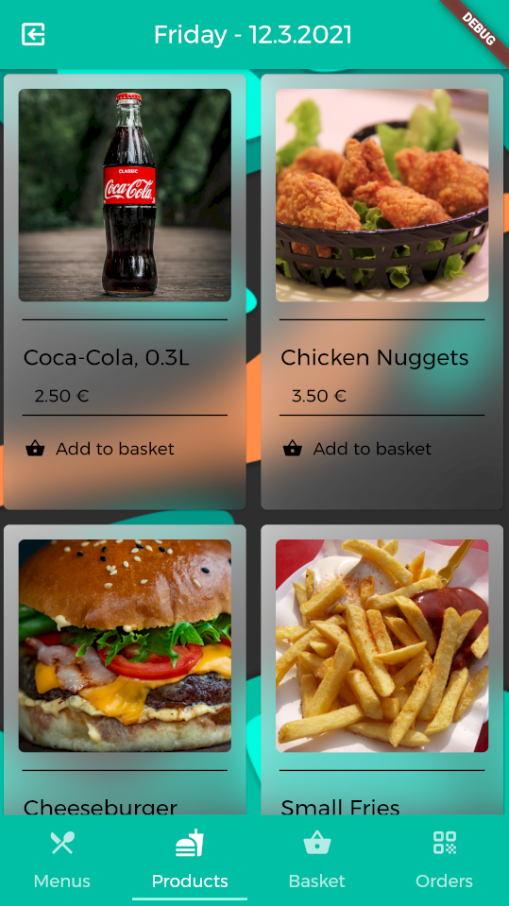
\includegraphics[width=0.40\textwidth]{images/Client/views/productview/productview.png}
    \caption{Product-View mit Kachel für das jeweilige Produkt}
\end{figure}

\subsection{Darstellen der Product-Tiles}

Für das Darstellen der einzelnen Product-Tiles wird das Open-Source \textit{flutter\_staggered\_grid\_view}-Package
verwendet. \cite{flutterStaggeredGridView}

Mithilfe dieser Library lässt sich einfach ein Grid-View mit dynamischen Reihen- und 
Spaltendimensionen definieren.

\begin{figure}[H]
    \centering
    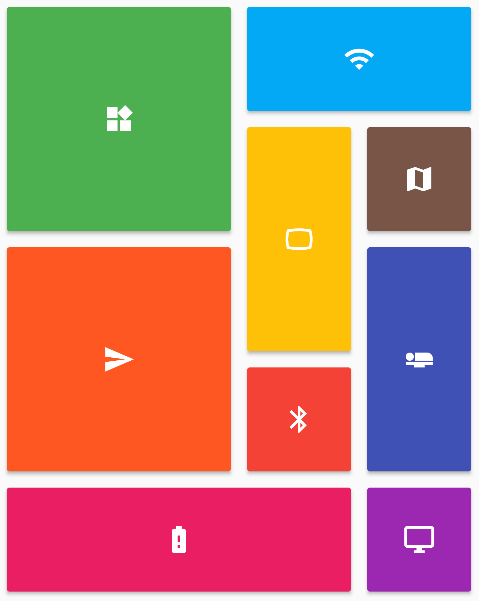
\includegraphics[width=0.5\textwidth]{images/Client/views/productview/staggeredGrid.png}
    \caption{Beispiel für ein Staggered-Grid-View \cite{flutterStaggeredGridViewImage}}
\end{figure}

Nun kann man im eigentlichen View für die Produktansicht mithilfe eines
\lstinline{StaggeredGridView.countBuilder}-Widgets die diversen Kacheln für alle vorrätigen Produkte
erstellen und anzeigen.

\begin{code}[H]
    \centering
    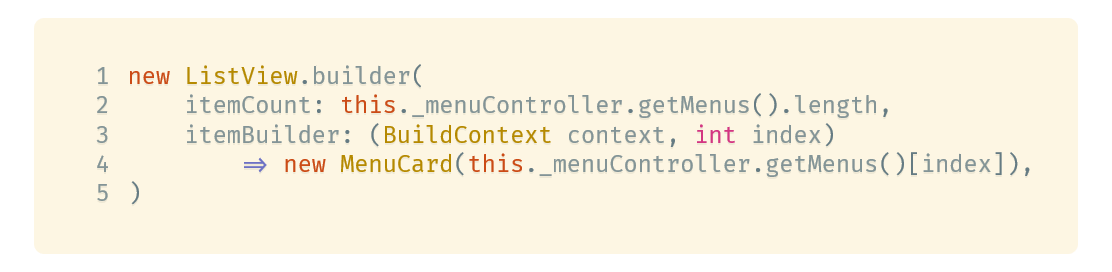
\includegraphics[width=1\textwidth]{images/Client/views/menuview/menuListViewBuilder.png}
    \vspace{-20pt}
    \caption{StaggeredGridView.countBuilder-Widget zum Erzeugen und Darstellen der Product-Tiles}
\end{code}

\newpage